
\clearemptydoublepage
\chapter{Attacks}
This chapter provides a comprehensive overview of system-level security threats in embedded systems. It begins by defining the concept of an attack and distinguishes between two primary categories: software attacks, which exploit vulnerabilities in code or system logic, and hardware attacks, which target the physical components of a system. 
\section{Definition}
With the rapid proliferation of embedded electronic systems in critical applications—ranging from automotive control units~\cite{7917080} and medical devices~\cite{4431854} to industrial automation and consumer electronics—their security has become a major concern. These systems often operate in environments where reliability and integrity are paramount, yet they are increasingly exposed to various threat vectors. As embedded systems grow in complexity and connectivity, they become attractive targets for attackers seeking to compromise system behavior, extract sensitive data, or cause functional disruption.

In this context, an attack is defined as any intentional act aimed at lowering the security level of an embedded system. Such acts may violate one or more core security properties: confidentiality, integrity, or availability. Attacks can be carried out through diverse methods, depending on the adversary’s access level, knowledge, and objectives. The origins of attacks in embedded systems trace back to early fault-tolerance~\cite{9684471} research, where hardware faults were studied for reliability purposes—later repurposed by adversaries as vectors for deliberate disruption. Over time, both hardware and software dimensions of these systems have revealed exploitable vulnerabilities.

Attacks are generally classified into two major categories: hardware attacks \cite{6856140} and software attacks \cite{6832045}. As Figure\ref{tree} shows, hardware attacks target the physical components of a system and include techniques such as fault injection, side-channel analysis, and probing. A comparison between hardware attacks and software Attack is shown in Table\ref{hw sw}. These methods typically require physical access but can be highly effective in bypassing traditional protections. Software attacks, on the other hand, exploit weaknesses in code, configuration, or system logic—examples include buffer overflows, code injection, and control-flow hijacking. Despite the differing methods, both types can produce system-wide effects and are therefore studied collectively under the broader category of system-level attacks.

\begin{figure}[t!]
  \centering
  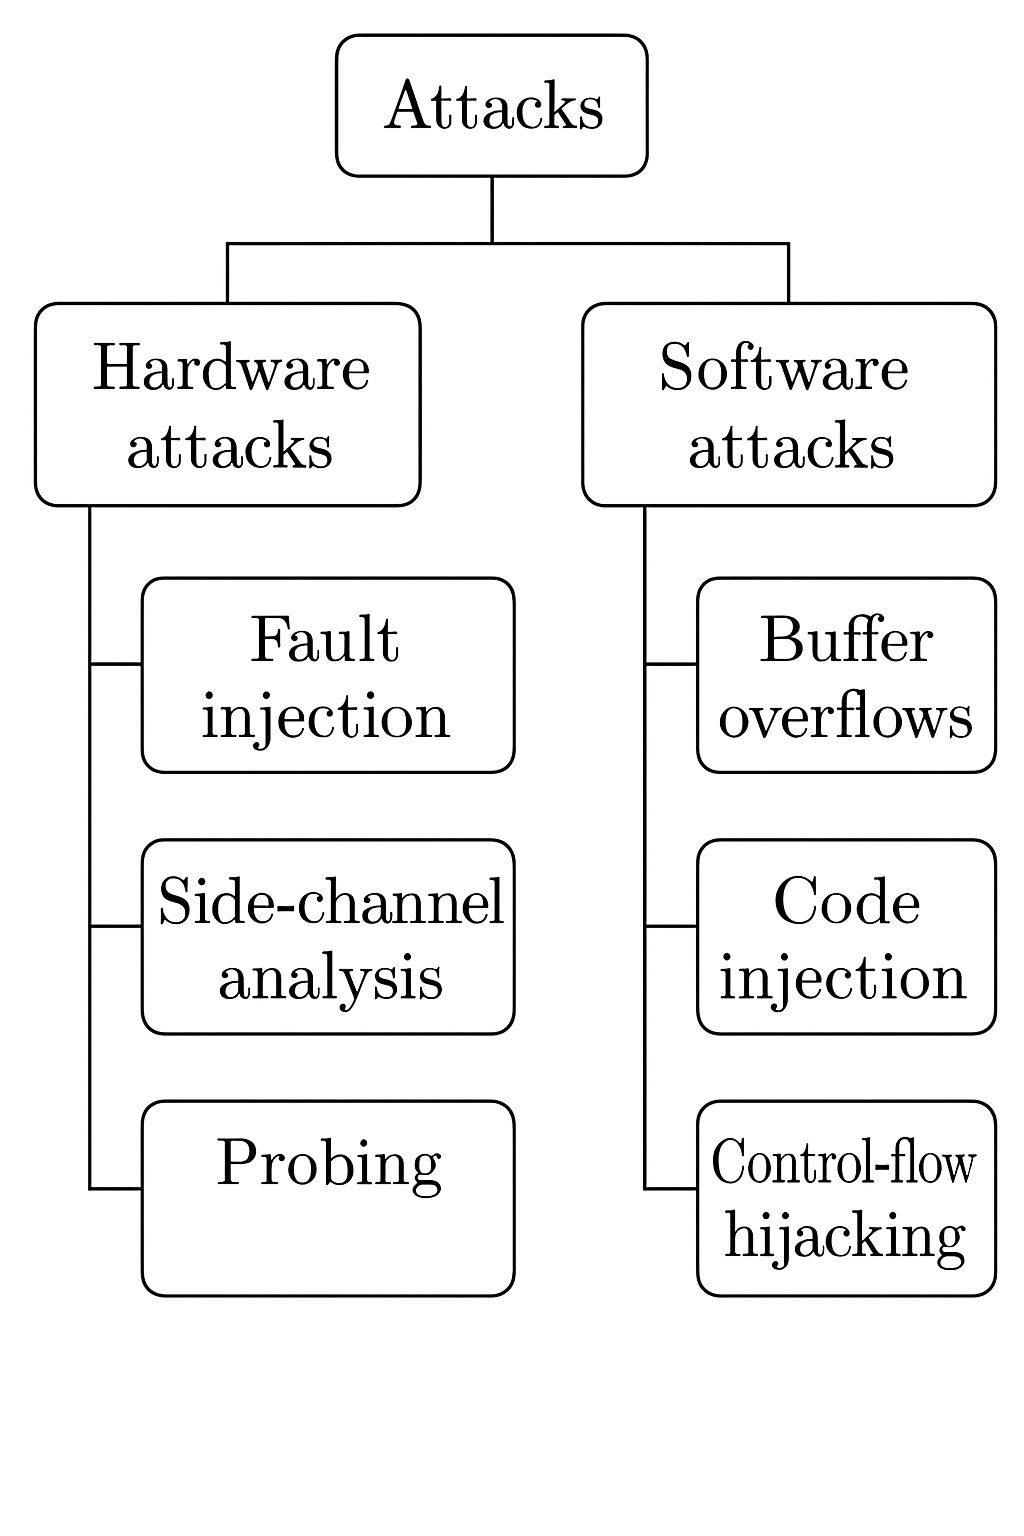
\includegraphics[width=0.5\linewidth]{Chapitre1/figures/tree.png}
  \caption{Classification of attacks into hardware and software categories, with representative techniques for each}
  \label{tree}
\end{figure}

\begin{table}[htbp]
\caption{Comparison of characteristics between hardware attack and software attack}
\label{hw sw}
\centering
\begin{tabularx}{\textwidth}{lXX}
\toprule
Aspect          & Hardware Attack                                          & Software Attack                                    \\
\midrule
Target Layer    & Physical components (CPU, memory, bus)                   & Software stack (code, memory, OS)                  \\
Access Method   & Requires physical or near-physical access                & Often remote, via crafted inputs or interfaces     \\
Techniques      & Fault injection, side-channel, probing                   & Buffer overflow, code injection, control hijacking \\
Detectability   & Hard to detect; minimal digital footprint                & Easier to monitor with logs and security tools     \\
Countermeasures & Costly and hard to retrofit; involve hardware redundancy & Easier to update via patches and software defenses \\
Typical Use     & Cryptographic key extraction, device tampering           & Privilege escalation, malware deployment           \\
\bottomrule
\end{tabularx}
\end{table}

\section{Software attack}
\subsection{Introduction and Classification}
In the domain of embedded and cyber-physical systems, software attacks \cite{6832002} constitute one of the most prevalent and evolving classes of security threats. Unlike hardware-based attacks, which typically require physical proximity or invasive access to a device, software attacks exploit logical vulnerabilities in code, configuration, or execution flow to subvert system behavior, escalate privileges, or extract sensitive data. These attacks are particularly insidious due to their ease of propagation, adaptability, and potential to be launched remotely.

From a classification perspective, software attacks on embedded systems can be categorized based on the attack vector, operational phase, or targeted system component. Broadly speaking, these can be delineated into:

\textbf{Code-level attacks}, such as memory corruption~\cite{1467812} and buffer overflows~\cite{821514}, exploit programming errors in memory management. These vulnerabilities allow attackers to manipulate control data structures—such as return addresses as shown in Figure \ref{buffer} or function pointers—to hijack the execution flow or inject arbitrary code. Since many embedded systems are implemented in memory-unsafe languages like C, these attacks remain a prevalent and potent threat.

\begin{figure}[t!]
  \centering
  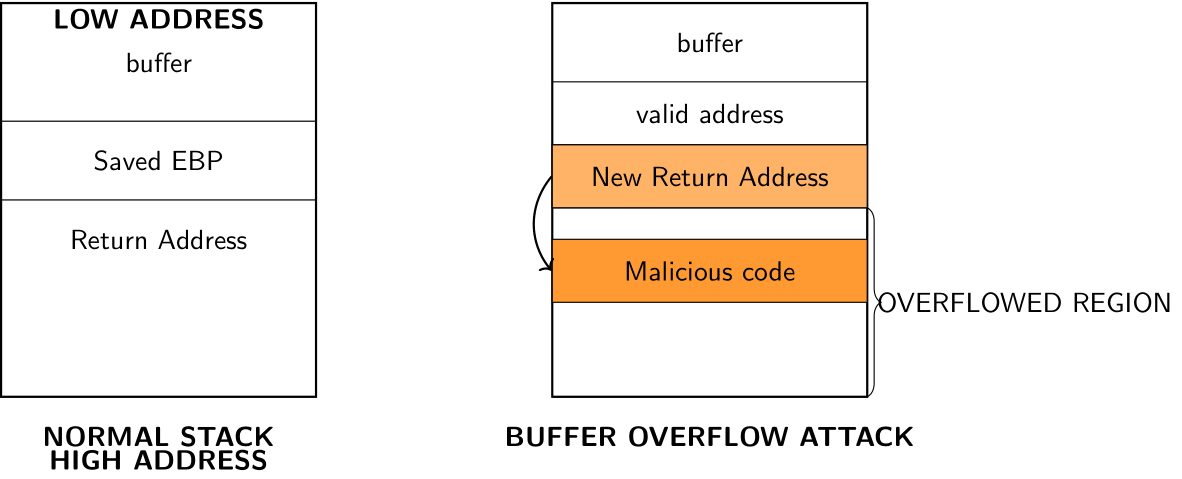
\includegraphics[width=0.5\linewidth]{Chapitre1/figures/buffer overflow.png}
  \caption{Principle of buffer overflow in program}
  \label{buffer}
\end{figure}

\textbf{System-level attacks} aim at compromising the trusted computing base of the system by targeting components such as operating system calls~\cite{9251949}, kernel modules~\cite{chen2011linux} and device drivers~\cite{yuce2018fault}, as shown in Figure\ref{system}. By exploiting these privileged layers, adversaries can gain access to critical resources, override security policies, or disable protection mechanisms entirely. These attacks are particularly dangerous due to their deep integration with the system architecture and wide-reaching consequences.

\begin{figure}[t!]
  \centering
  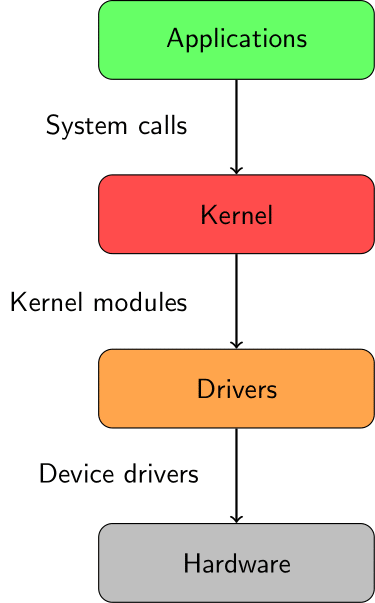
\includegraphics[width=0.5\linewidth]{Chapitre1/figures/system.png}
  \caption{Different system-level attack aspects}
  \label{system}
\end{figure}

\textbf{Firmware manipulation} involves tampering with the low-level binary code responsible for device initialization and hardware configuration. Typical targets include bootloaders~\cite{redini2017bootstomp} and embedded system images~\cite{ling2023adversarial}, which can be modified to introduce persistent malicious behavior as Figure \ref{Firmware} shows. Firmware-level attacks are often stealthy and durable, capable of surviving system resets and bypassing runtime protections.

\begin{figure}[t!]
  \centering
  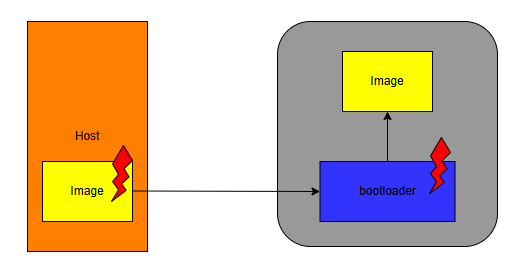
\includegraphics[width=0.5\linewidth]{Chapitre1/figures/Firmware.png}
  \caption{Firmware manipulation on bootloader and embedded system image}
  \label{Firmware}
\end{figure}

\textbf{Malicious configuration} and \textbf{runtime reprogramming} represent another class of attacks that do not directly alter code but instead manipulate system behavior by changing initialization values, parameter tables, or control logic at runtime~\cite{sinanovic2017analysis, alam2020soft}. As the Figure shows, the attacker can change initial value of a as 4,  These methods can bypass traditional integrity checks and allow adversaries to exploit dynamic features of embedded systems, such as reconfigurability or exposed debugging interfaces.

\begin{figure}[t!]
  \centering
  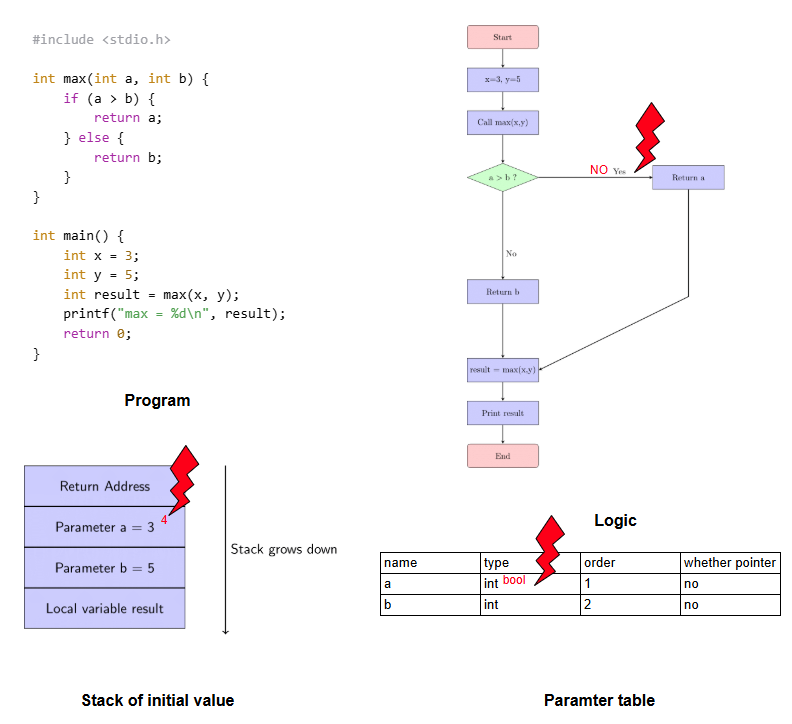
\includegraphics[width=0.5\linewidth]{Chapitre1/figures/malicious.png}
  \caption{Malicious configuration by changing initialization values, parameter tables and control logic}
  \label{malicious}
\end{figure}

\textbf{Application-level exploitation} targets flaws in application logic or communication interfaces. Common techniques include exploiting improper input validation~\cite{hayati2008modeling}, abusing insecure update procedures~\cite{alhamed2013stacking}, or leveraging weak authentication mechanisms. These attacks often serve as entry points for more persistent compromises, especially in systems that lack isolation between application and system layers.

Each class of software attack can be further analyzed along several dimensions, allowing for a more structured understanding of their mechanisms and implications. One key dimension is the attacker’s knowledge model, which refers to the level of internal system knowledge available to the adversary. In a black-box model, the attacker has no information about the system’s internal architecture or behavior and relies solely on observed input-output relationships. In contrast, the white-box model assumes complete knowledge of the system, including source code, memory layout, and execution environment. The gray-box model lies in between, where partial information is available—such as known APIs or hardware specifications—allowing for more targeted attacks without full system access.

Another important classification criterion is the delivery method of the attack. Software attacks may be introduced through various channels, depending on system accessibility and vulnerability exposure. These include over-the-air updates, which can be exploited to inject malicious firmware or configuration changes; local scripts or binaries, often executed through command-line interfaces or operating system vulnerabilities; and interface fuzzing, where malformed or randomized inputs are sent to system interfaces (e.g., I/O ports, communication buses, or APIs) to trigger unintended behaviors.

Finally, software attacks can also be distinguished by their persistence goal. Some aim for temporary disruption, such as inducing transient faults or causing momentary denial-of-service conditions \cite{7081075}. Others pursue long-term compromise, seeking to establish persistent control over the system—for example, by injecting backdoors \cite{tol2022toward}, modifying firmware \cite{bettayeb2019firmware}, or escalating privileges \cite{davi2010privilege}.

Understanding this multi-dimensional taxonomy of software attacks is essential for several reasons. It enables the development of more comprehensive threat models, facilitates risk assessment at different levels of the system, and informs the design of tailored defense mechanisms that can address a wider spectrum of threats across different attack surfaces and adversary capabilities.

\subsection{Attack Methodologies}
Software attacks exploit logical vulnerabilities, design flaws, or execution behaviors within a system’s software stack to compromise confidentiality, integrity, or availability. These attacks often bypass hardware-level defenses by manipulating code execution, system memory, or control flow at various abstraction levels. Over the past decades, software attack methodologies have evolved in sophistication—from early buffer overflows to modern fault-induced logic corruption—driven by advancements in both attack tools and target complexity.

One of the most fundamental classes of software attacks involves control-flow manipulation, where an adversary seeks to alter the intended execution path of a program. Techniques such as return-oriented programming (ROP)\cite{checkoway2010return}, jump-oriented programming (JOP)\cite{bletsch2011jump}, and function pointer hijacking \cite{bertani2023untangle} allow attackers to redirect the flow of execution without injecting new code. These methods rely on the ability to overwrite stack or heap structures, often through memory corruption vulnerabilities like buffer overflows or use-after-free conditions.

Closely related are code injection attacks, where malicious code is introduced into the memory space of a running process. Historically, these attacks were prevalent in systems lacking execution protection (e.g., DEP\cite{isawa2013generic}/NX\cite{werner2016no}), where attacker-controlled data could be both written and executed. While modern architectures implement various memory protections, code injection remains feasible when combined with information leakage or runtime reconfiguration, such as just-in-time (JIT) spraying \cite{chen2013jitsafe} or script-based code assembly \cite{wang2013metasymploit}.

Another important category includes privilege escalation \cite{davi2010privilege} and logical bypass attacks \cite{xu2017novel}, where adversaries exploit incorrect access control implementations or faulty assumptions in system logic. These attacks may be local—e.g., escalating from user to kernel space—or remote, targeting web-based interfaces or firmware. A fault injection at the software level, such as skipping an authentication check or corrupting return values, can directly result in unauthorized privilege gains.

An increasingly relevant methodology involves fault-assisted software attacks \cite{yuce2018fault}, which blur the boundary between physical disturbance and logical manipulation. By inducing faults—via electromagnetic pulses, clock/voltage glitches, or even rowhammer-style memory perturbations—attackers can corrupt specific instructions, modify control variables, or cause inconsistent system states. This type of attack has been successfully used to bypass cryptographic checks, tamper with authentication logic, or induce incorrect branching decisions. Importantly, such attacks exploit the dynamic behavior of executing software rather than static vulnerabilities.

Micro-architectural exploitation, including techniques like Spectre, Meltdown, and more recently transient execution attacks, represents another powerful software-level methodology. These attacks leverage speculative execution and cache side-effects to leak data across security boundaries, without violating any formal access rules. Although the attack surface lies in software instructions, the underlying vulnerabilities are deeply rooted in hardware optimizations, making them challenging to fully mitigate.

Additionally, software fault injection (SFI) frameworks \cite{9251063} have been developed not only for testing purposes but also as practical tools for controlled attack simulation. These frameworks can be used to corrupt instruction execution, memory accesses, or system calls by injecting faults through software instrumentation, binary rewriting, or emulator-level fault triggers. Such tools have been used both by attackers to explore system behavior under fault conditions, and by defenders to evaluate the robustness of their software under adversarial scenarios.

In summary, software attack methodologies encompass a wide spectrum of techniques, from traditional memory corruption to advanced fault-assisted logic manipulation and micro-architectural abuse. These methods often require little or no physical access to the system and can operate remotely, making them particularly dangerous in networked or IoT environments. As software continues to serve as the interface between users and hardware, understanding the diversity and evolution of these attacks remains essential for the development of resilient systems.

\subsection{Countermeasures}
To address software attack vectors—particularly those exploiting faults during execution—researchers have developed a diverse set of countermeasures grounded in three core principles: redundancy, isolation, and desynchronization. These principles serve as the foundation for both theoretical frameworks and practical implementations that aim to increase the resilience of software and hardware systems under adversarial conditions.

\textit{Detection and correction} methods rely on introducing various forms of redundancy to detect or recover from the effects of injected faults. Modular redundancy~\cite{dutertre2011review} replicates functional modules and compares their outputs at runtime to identify discrepancies. This strategy is especially effective in critical systems where reliability is paramount, such as aerospace or medical applications. Time redundancy~\cite{manssour2022processor} leverages the re-execution of operations across different clock cycles, under the assumption that transient faults are unlikely to repeat identically. While computationally more expensive, this approach is often suitable for safety-critical tasks. Information redundancy, such as cyclic redundancy checks (CRC), parity bits, or Hamming codes~\cite{yuce2016fame}, embeds fault detection directly into the data path, enabling automatic identification of corrupted values. However, all these methods remain vulnerable to correlated fault injections, especially when attackers synchronize faults across duplicated resources, potentially rendering detection mechanisms ineffective.

\textit{Isolation techniques} aim to physically or logically decouple vulnerable components from potential sources of disturbance. Beyond conventional software-based isolation such as process separation and memory protection, recent advancements leverage hardware-assisted environments to construct trustworthy execution domains. These enhanced mechanisms, including Trusted Execution Environments (e.g., ARM TrustZone\cite{pinto2019demystifying}, Intel SGX\cite{mckeen2016intel}), secure enclaves\cite{beekman2016improving}, and hypervisor-based isolation\cite{hua2012barrier}, allow sensitive code to run in contexts that are logically and physically separated from the main operating system. While not purely software constructs, they fulfill the role of high-assurance software isolation by enforcing strict execution boundaries that fault injection attempts cannot easily traverse.

\textit{Desynchronization} counters fault attacks by reducing temporal predictability, thereby making it harder for attackers to align fault injections with critical execution phases. Techniques in this domain include randomizing internal clock frequencies, injecting random delays, or dynamically altering the order of instruction execution~\cite{patrick2017lightweight, wang2016against}. Dummy instructions—operations that do not contribute to program logic but consume time—are also commonly used to obscure program behavior and confuse attackers. However, the effectiveness of desynchronization can be undermined by advanced fault characterization techniques such as Fault Intensity Map Analysis (FIMA) \cite{ramezanpour2019fima} or Statistical Ineffective Fault Attacks (SIFA) \cite{dobraunig2018statistical}, which exploit aggregate fault behavior to infer fault locations or reduce entropy in randomized systems.

Building on these architectural concepts, numerous practical \textbf{software-level} countermeasures have been proposed. Compiler-assisted approaches, such as those built on the LLVM framework, can automate the insertion of fault-tolerant constructs like instruction duplication, control flow verification, or consistency checks~\cite{Barry2016}. Cryptographic routines, which are high-value targets in many systems, are frequently hardened through redundant calculations and integrity checks that validate intermediate results~\cite{Barenghi2010}. In contexts where source code is unavailable or legacy binaries must be secured, binary rewriting techniques provide a powerful alternative. These approaches inject countermeasure logic directly into compiled executables~\cite{Kiaei2021}, allowing defenses to be deployed post-compilation without altering original development pipelines.

On the \textbf{hardware level}, defenses are increasingly embedded directly into the CPU and its execution pipeline. Fault-tolerant decoders equipped with parity or checksum validation can detect faults in instruction fetch and decode stages~\cite{Shukla2023}. Register file protection has also been explored through techniques that remap sensitive data into distributed memory cells combined with parity-based integrity checking~\cite{Ramos2018}. These strategies allow low-overhead error detection while preserving performance and compatibility with existing toolchains.

Control-flow integrity (CFI) mechanisms offer another line of defense against fault-induced diversions in execution. The CIFER system~\cite{zgheib2023cifer} integrates runtime code integrity and control-flow verification on RISC-V processors, protecting against instruction skipping and code modification. SCI-FI~\cite{chamelot2022scifi} extends this idea by targeting both software logic and hardware control signals, making it more resilient to low-level fault attacks. Instruction stream encryption~\cite{werner2019riscv}, implemented via an additional pipeline stage, ensures that fault-induced control flow diversions are rendered ineffective unless the encryption state is preserved. Other research~\cite{nasahl2021arm} proposes refined CFI updates that protect dynamic branches and indirect jumps, which are particularly vulnerable to control hijacking under fault conditions.

In terms of \textbf{memory protection}, researchers have focused on defending address resolution and access logic from corruption. The SecWalk architecture~\cite{Schilling2021} provides comprehensive protection for virtual memory translation, safeguarding page table walks against injected faults that aim to redirect or invalidate memory accesses. Complementary work~\cite{Schilling2018} introduces runtime memory access verification mechanisms that monitor and validate each memory operation against expected access patterns, thus detecting anomalies caused by fault injection in memory controllers or instruction decoders.

In summary, countermeasures against software-level fault attacks encompass a broad spectrum of techniques—from code transformation and compiler-level defenses to on-chip architectural protections and memory access validation. While none of these solutions is universally effective against all fault models, their combined application significantly raises the difficulty and cost of successful attacks. As fault injection continues to evolve toward more precise, high-resolution methods, the development of multi-layered and cross-domain countermeasures remains an essential research direction for securing embedded and cyber-physical systems.

\section{Hardware attack}
\subsection{Introduction and Classification}
Hardware attacks refer to malicious actions that exploit the physical characteristics or structural implementation of integrated circuits (ICs) and electronic systems in order to compromise their confidentiality, integrity, or availability. Unlike software attacks, which manipulate code or logic at an abstract level, hardware attacks interact directly with the physical substrate of a system, making them capable of bypassing software-based protections and revealing sensitive internal states that would otherwise be inaccessible. Several categories of hardware attacks have been identified in the literature, each employing distinct techniques and targeting different stages of the hardware lifecycle.

Reverse Engineering \cite{varady1997reverse}, as Figure\ref{malicious} is the process of extracting a device’s internal design or functionality through direct observation and analysis. This may involve delayering an integrated circuit to image its layers, reconstructing its gate-level netlist, or recovering embedded firmware from non-volatile memory. Reverse engineering is often used as a precursor to more advanced attacks or for intellectual property (IP) theft, and may be performed invasively or non-invasively depending on the desired resolution and access.

\begin{figure}[t!]
  \centering
  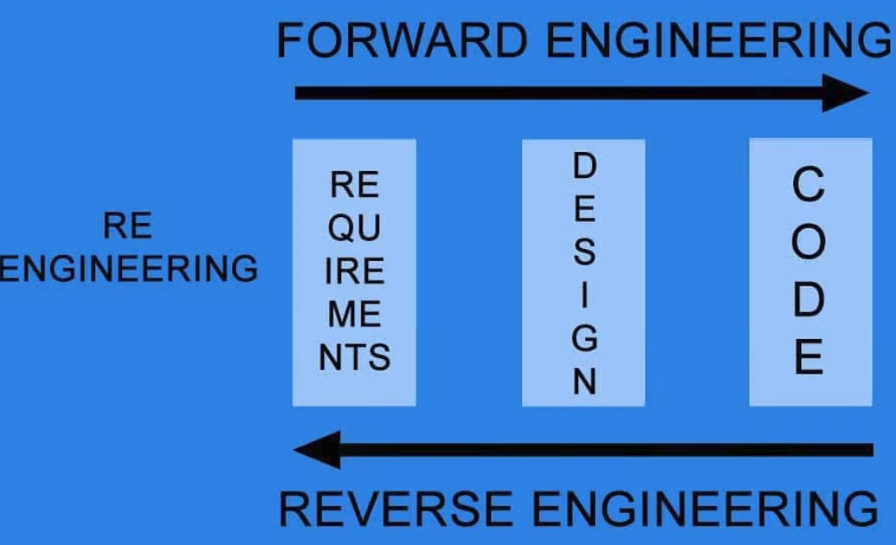
\includegraphics[width=0.5\linewidth]{Chapitre1/figures/reverse.png}
  \caption{Reverse engineering procedure (source: \url{https://t2informatik.de/en/smartpedia/reverse-engineering/})}
  \label{malicious}
\end{figure}

Fault Injection Attacks (FIA) \cite{hsueh1997fault} involve deliberately inducing faults into the hardware with the goal of altering its normal behavior(as Figure \ref{fault injection}). These faults can be transient or permanent and may be introduced through methods such as voltage glitches, clock disturbances, electromagnetic pulses, laser beams, or thermal stress. By causing errors in computation or control flow, attackers can bypass security checks, extract secret information, or compromise critical functions. FIA represents a powerful attack vector, particularly because it operates at the boundary between physical disturbance and software response.

\begin{figure}[t!]
  \centering
  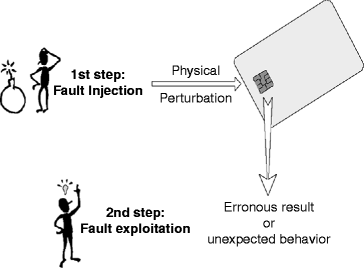
\includegraphics[width=0.5\linewidth]{Chapitre1/figures/fault.png}
  \caption{Fault injection procedure (source: \url{https://link.springer.com/rwe/10.1007/978-1-4419-5906-5_505})}
  \label{fault injection}
\end{figure}

Side-Channel Attacks (SCA) \cite{kelsey1998side} as Figure\ref{side channel attack} exploit information that leaks unintentionally during the normal operation of a device. These leaks can manifest as variations in power consumption, electromagnetic emissions, timing behavior, or even acoustic signals. By observing and analyzing these physical side effects, attackers can infer secret data such as cryptographic keys or internal program states. Unlike fault injection, SCA does not aim to alter system behavior, but rather to passively observe it with high precision.

\begin{figure}[t!]
  \centering
  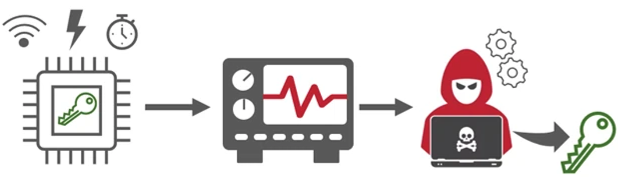
\includegraphics[width=0.5\linewidth]{Chapitre1/figures/sca.png}
  \caption{Side-Channel Attacks procedure (source: \url{https://semiengineering.com/secure-your-soc-from-side-channel-attacks-with-adaptable-security/})}
  \label{side channel attack}
\end{figure}

Hardware Trojan Insertion \cite{chakraborty2009hardware} as Figure \ref{hardware trojan} refers to the deliberate embedding of malicious logic within a hardware design. This can occur during design, fabrication, or post-fabrication stages, often without detection. Hardware Trojans may remain dormant until triggered by specific conditions, at which point they can leak information, degrade performance, or disable functionality. Their stealthy nature and integration within legitimate hardware make detection and prevention especially challenging.

\begin{figure}[t!]
  \centering
  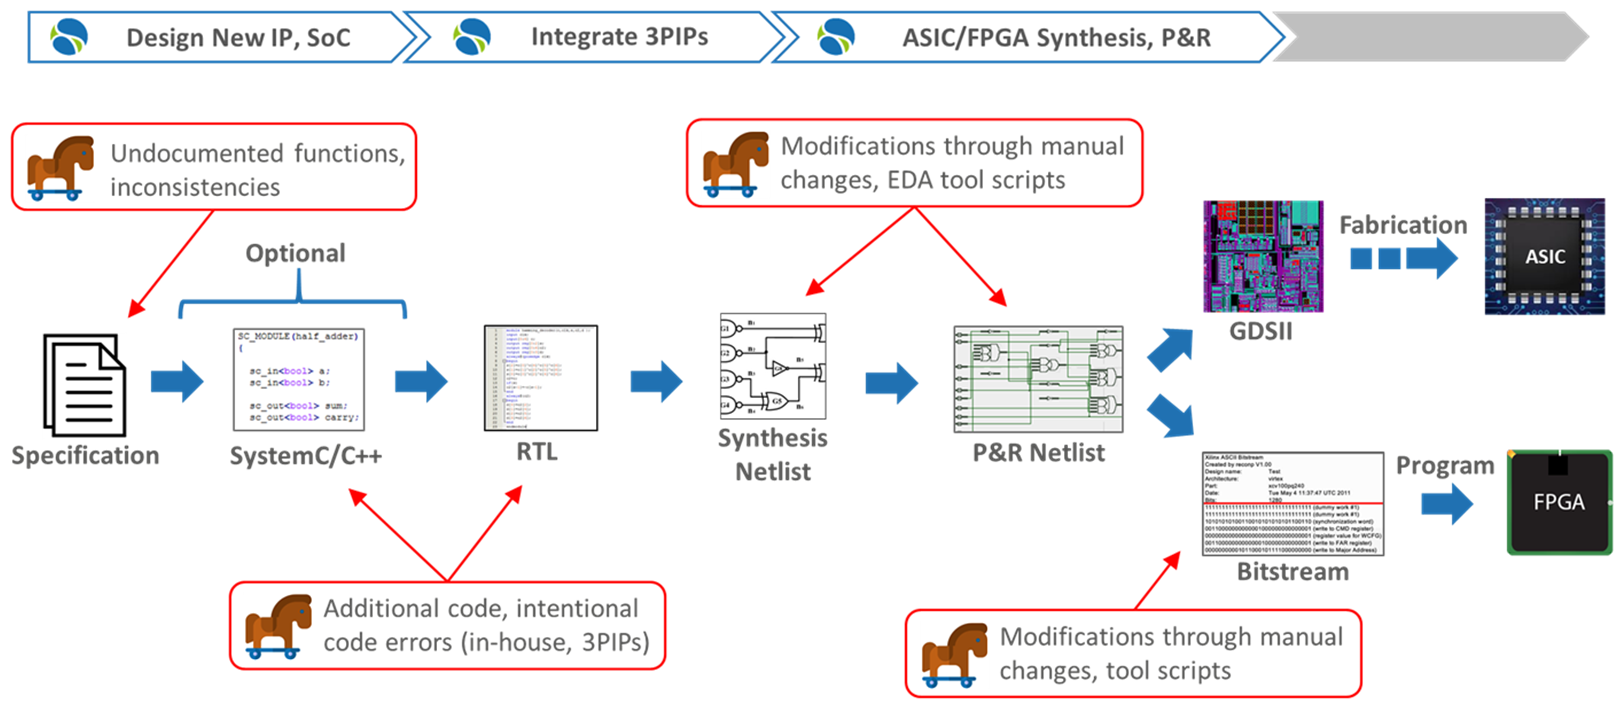
\includegraphics[width=0.5\linewidth]{Chapitre1/figures/hardware trojan.png}
  \caption{Hardware Trojan Insertion procedure (source: \url{https://semiengineering.com/hardware-trojans-and-the-problem-of-trust-in-integrated-circuits/})}
  \label{hardware trojan}
\end{figure}

\subsection{Fault Injection methods}

Clock fault injection (Figure \ref{clock fault}) can be achieved through several mechanisms, including manipulating the clock period, introducing voltage disturbances, or intentionally reducing the power supply. In the case of clock manipulation, reducing the clock period may result in insufficient setup time for certain signal paths, causing data to arrive at flip-flops too late relative to the clock edge. This misalignment can lead to erroneous values being captured. An early implementation of this technique was presented by Agoyan et al. \cite{agoyan2010clocks}, who targeted an AES encryption core implemented on an FPGA with a delay-locked loop (DLL)-based clocking system. Similar results were reported in \cite{selmke2019peak}, where externally induced glitches affected the clock signal of an ARM-based microcontroller, even though the internal system clock was derived from a phase-locked loop (PLL), illustrating the vulnerability of PLL-based systems to external perturbations.

\begin{figure}[t!]
  \centering
  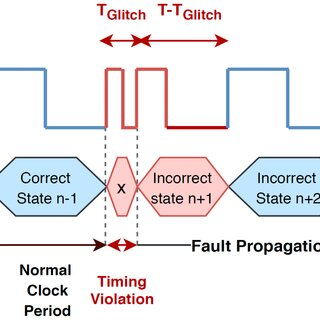
\includegraphics[width=0.5\linewidth]{Chapitre1/figures/clock fault.jpg}
  \caption{Clock fault principle (source: \url{https://www.researchgate.net/figure/Representation-of-clock-glitch-and-fault-injection-17_fig4_343027498})}
  \label{clock fault}
\end{figure}

Voltage-based fault injection methods (Figure \ref{voltage fault}) exploit the delay characteristics of CMOS circuits under reduced supply conditions. By introducing brief voltage drops or operating the device under nominal voltage thresholds, attackers can increase the signal propagation delay within the combinational logic. This delay may prevent correct evaluation before the next clock edge, thereby injecting computation faults. Selmane et al. \cite{selmane2008practical} demonstrated this principle in a practical attack scenario, where underpowering a smart card executing AES operations resulted in faulty outputs. Later investigations, such as the one conducted by Zussa et al. \cite{zussa2013power}, examined the impact of negative voltage pulses on FPGA implementations. Their findings indicated that the observable fault patterns induced by power glitches closely resemble those caused by clock manipulation, suggesting a convergence in their physical effects.

\begin{figure}[t!]
  \centering
  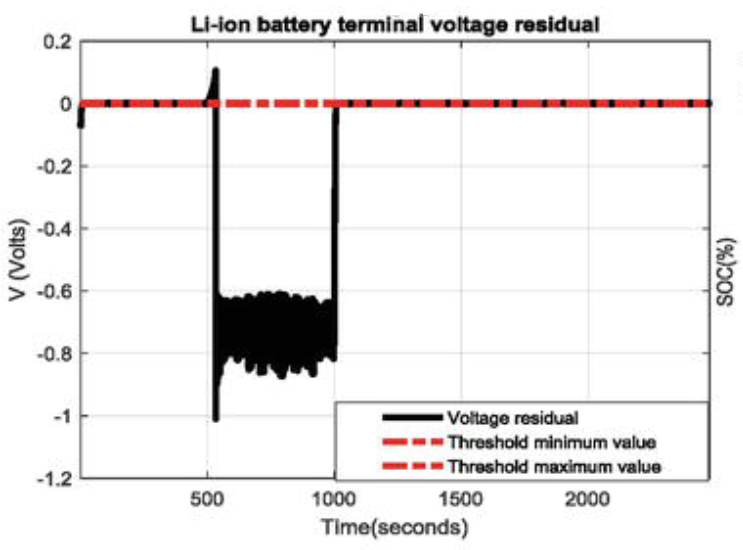
\includegraphics[width=0.5\linewidth]{Chapitre1/figures/voltage.png}
  \caption{Voltage fault waveform (source: \url{https://www.intechopen.com/chapters/74031})}
  \label{voltage fault}
\end{figure}

Electromagnetic (EM) (Figure \ref{electromagnetic fault}) interference represents another class of fault injection, relying on the alteration of timing relationships within the circuit \cite{trouchkine2021electromagnetic} ~\cite{trouchkine2021fault}. When exposed to strong EM fields, the synchronization between clock signals and data lines can be disturbed. As a result, bits stored in memory cells or registers may be erroneously set or reset. This form of attack was pioneered by Quisquater et al. ~\cite{quisquater2002eddy}, who demonstrated that applying electromagnetic perturbations to various memory technologies could induce fault conditions in a contactless and localized manner. In this paper~\cite{sass2023oops}, they present \textmu-Glitch, the first Voltage Fault Injection (VFI) platform which is capable of injecting multiple, coordinated voltage faults into a target device, requiring only a single trigger signal. Their evaluation revealed that \textmu-Glitch can successfully inject four consecutive faults within an average time of one day.

\begin{figure}[t!]
  \centering
  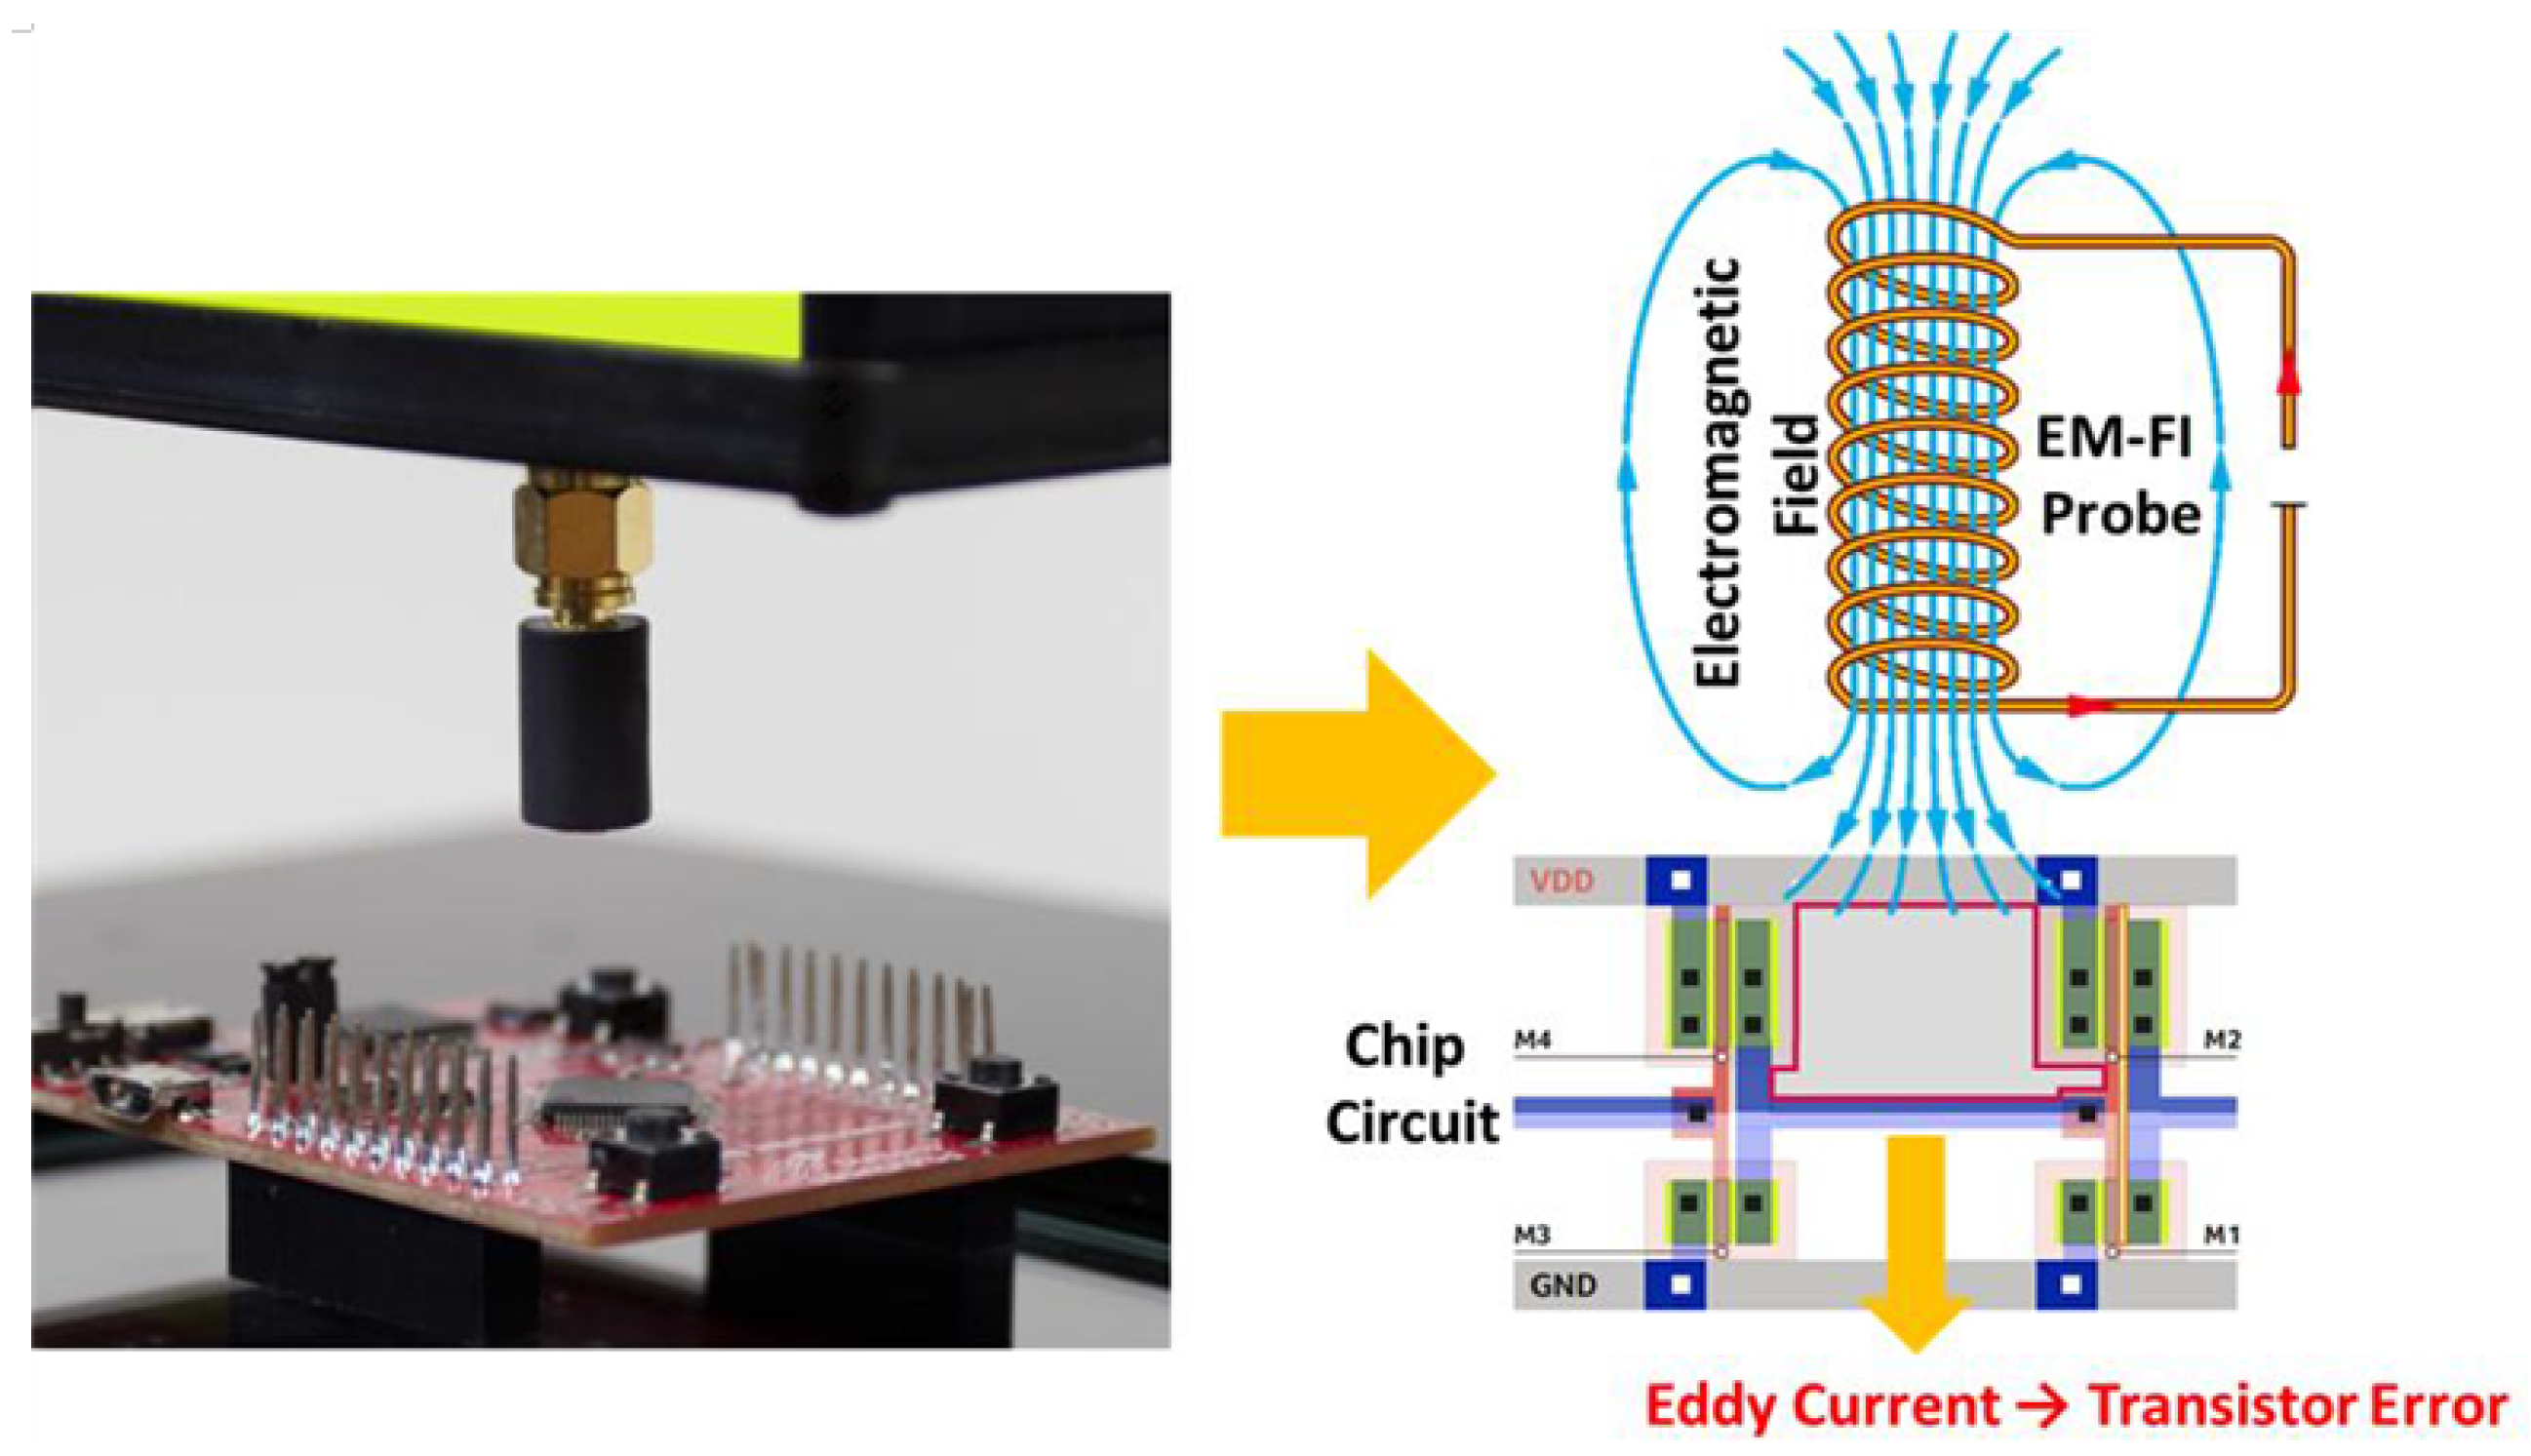
\includegraphics[width=0.5\linewidth]{Chapitre1/figures/em.png}
  \caption{Electromagnetic fault principle (source: \url{https://www.researchgate.net/figure/Representation-of-clock-glitch-and-fault-injection-17_fig4_343027498})}
  \label{electromagnetic fault}
\end{figure}

Optical injection techniques (Figure \ref{optical fault}) provide finer spatial resolution. The first optical fault injection attack was proposed by Skorobogatov and Anderson~\cite{skorobogatov2003optical}, where they utilized a photographic flash to disturb SRAM cells in microcontrollers. This approach exploits the light sensitivity of semiconductor materials, where photons generate transient charge carriers that alter the state of logic gates or memory elements. More advanced implementations later used focused laser beams to achieve precise control over the affected region, allowing faults to be targeted at specific registers or datapaths.

\begin{figure}[t!]
  \centering
  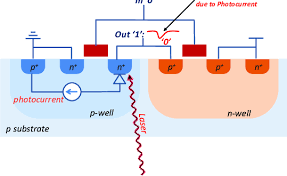
\includegraphics[width=0.5\linewidth]{Chapitre1/figures/laser.png}
  \caption{Laser fault attack on CMOS (source: \url{https://www.researchgate.net/figure/Laser-Fault-Injection-LFI-mechanism-in-the-case-of-a-simple-CMOS-inverter_fig1_376090023})}
  \label{optical fault}
\end{figure}

In addition to the techniques mentioned above, fault injection through body biasing and X-ray irradiation has also been explored. Body biasing alters the threshold voltage of transistors by adjusting the substrate potential, thereby increasing the susceptibility of certain regions to timing violations. This was demonstrated in the work of Tobich et al. \cite{tobich2012yet} and later refined by O'Flynn et al. \cite{o2021low}. On the other hand, nanofocused X-ray beams have been proposed as a means to disturb circuit behavior at the atomic scale. Anceau et al.~\cite{anceau2017nanofocused} investigated the feasibility of this method, showing that localized exposure can lead to significant disruption in device functionality, although the technique currently remains within the domain of laboratory-scale experiments.

\subsection{Fault Injection Hierarchy}
Fault injection attacks can be understood across several abstraction layers of a computing system, from high-level software instructions down to the physical behavior of transistors. This hierarchical view is essential for understanding the range of possible effects a fault may induce, as well as for designing appropriate countermeasures.

At the \textit{instruction level}, attackers aim to corrupt the program’s control flow or logic by targeting the encoding of instructions. One common strategy is instruction skipping, where the execution of one or more instructions is prevented, effectively bypassing conditional checks or security validations~\cite{alshaer2022cross, dehbaoui2013electromagnetic}. In more complex scenarios, attackers have demonstrated the ability to skip multiple consecutive instructions~\cite{riviere2015high, nashimoto2017buffer}, or to cause a single instruction to be executed repeatedly or replaced with a different operation~\cite{khuat2021laser, alshaer2022variable, balasch2011depth, timmers2016controlling}. These manipulations alter the intended meaning of the program without modifying the binary, which makes them difficult to detect through static analysis alone.

At the \textit{micro-architectural level}, faults interact with internal processor components such as pipeline stages, register files, and cache hierarchies. These attacks disrupt implicit hardware assumptions about timing, resource arbitration, or speculative execution. For instance, faults can interfere with instruction decoding or pipeline forwarding logic, leading to unintended execution paths or stale data propagation~\cite{Tollec2022exploration}. Micro-architectural-level effects are often more difficult to model, as they depend on the specific implementation of the processor, including undocumented behaviors or vendor-specific optimizations.

At the \textit{circuit level}, attackers target the electrical properties of the digital logic itself. By manipulating signal propagation delays or altering the threshold voltage of transistors, an attacker may induce incorrect switching behavior in gates or flip-flops. This could result in bit flips, stuck-at faults, or randomization of signal values. Depending on the fault model, the effect may corrupt a single bit, a byte, or even entire registers or memory words—potentially affecting security-critical variables such as cryptographic keys or control flags~\cite{barenghi2012fault, marc2012fault}. Faults at this level can be induced using techniques such as voltage glitches, electromagnetic pulses, or laser irradiation, and typically require precise spatial and temporal alignment to be effective.

To comprehensively evaluate system resilience, it is important to understand how faults at lower levels of the hierarchy propagate to higher levels. For example, a transient fault at the transistor level may manifest as a corrupted instruction in the pipeline, which in turn may result in a logic bypass or privilege escalation at the software level. Therefore, defense strategies must be designed with cross-layer awareness, accounting for both the physical origin of faults and their logical consequences across abstraction boundaries.

\subsection{Fault Injection Countermeasure}
Despite the fact that multiple architectural layers remain vulnerable to fault injection attacks, a variety of defensive techniques have been developed to enhance system robustness. These countermeasures aim either to detect, withstand, or obscure the effects of injected faults, and are typically implemented at different abstraction levels. While none of these methods offer absolute protection, their combined application can significantly increase the difficulty of mounting a successful attack.

A first class of countermeasures focuses on \textit{fault detection and correction}, where the primary objective is to identify the occurrence of faults and respond appropriately. Most of these strategies rely on introducing some form of redundancy. For instance, hardware-level duplication—known as modular redundancy—executes the same operation in parallel on multiple instances of the same logic, with consistency checks performed on the outputs~\cite{dutertre2011review}. Alternatively, \textit{time redundancy} involves re-executing computations at different time intervals and comparing results~\cite{manssour2022processor}. At the data level, \textit{information redundancy} techniques, such as parity bits or error detection codes, are used to encode and verify the integrity of sensitive variables~\cite{yuce2016fame}~\cite{elbaz2009hardware}. However, these approaches can be circumvented if the injected fault affects multiple redundant elements simultaneously or occurs in such a way that errors cancel out across the comparison logic.

In parallel, \textit{isolation-based defenses} have proven effective in limiting the adversary's ability to physically interact with or influence the critical regions of a chip. One practical measure is the use of physical shielding, which encloses vulnerable zones of the device with protective layers to prevent optical, electromagnetic, or mechanical access~\cite{avital2024enhancing}. Another complementary technique involves signal \textit{filtering}, where components such as integrated voltage regulators or passive filters are inserted between external interfaces and the internal circuit to attenuate the impact of voltage glitches or electromagnetic transients~\cite{fanjas2022combined}. These forms of isolation are especially relevant when combined with tamper-evident packaging or sensor-triggered response logic~\cite{qi2016design}.

To further complicate the timing precision required for fault injection, many implementations incorporate \textit{desynchronization techniques}, sometimes referred to as temporal or architectural randomization. As for the software countermeasure, the core idea is to introduce unpredictability into the execution flow, making it more difficult for attackers to align their fault attempts with specific instruction boundaries or computation phases. This can be achieved by using non-deterministic internal clock sources, random delays, instruction shuffling, or injecting dummy operations~\cite{patrick2017lightweight, wang2016against}. While these techniques can greatly reduce fault success rates under brute-force conditions, more sophisticated attacks have emerged that exploit residual patterns. Notably, approaches such as Fault Intensity Map Analysis (FIMA) \cite{ramezanpour2019fima} and Statistical Ineffective Fault Attacks (SIFA) \cite{dobraunig2018statistical} use statistical modeling and spatial fault profiling to recover fault injection parameters, even in randomized environments.

Collectively, these countermeasures illustrate the ongoing arms race between fault injection techniques and defensive engineering. A robust defense strategy requires not only the layering of these countermeasures, but also a clear understanding of the attacker model, fault injection capabilities, and the system’s operational context.

\section{Studies Combining Hardware-Software Attacks}
In modern embedded systems, the boundary between hardware and software security is increasingly blurred. While hardware and software attacks are often studied separately, a growing body of research has demonstrated that combined hardware-software attack strategies—which exploit the interplay between physical-layer vulnerabilities and software-level logic—can significantly amplify the effectiveness and stealth of an attack. These hybrid techniques represent a sophisticated threat model that is particularly relevant in the context of complex SoC designs, where hardware, firmware, and application code interact tightly and often rely on shared resources and assumptions.

At their core, combined attacks exploit the physical ability to induce faults or extract side-channel information, while leveraging software logic or architectural knowledge to guide, refine, or interpret the results of such manipulation. This technique is particularly powerful in scenarios such as instruction skipping, faulting condition checks, or bypassing cryptographic authentication.

One of the most well-known examples of this combination is the fault attack on software-controlled cryptographic operations, where physical disturbances are introduced at precisely timed execution stages \cite{buhren2021one}. For instance, fault injection may be used to corrupt a register holding an intermediate value of an AES computation, and then a software routine may capture the faulty output and perform differential analysis to recover the secret key. Such attacks—e.g., DFA (Differential Fault Analysis) \cite{biham1997differential} —demonstrate how precise hardware faults can be exploited through structured software-level observation.

Another common form of combined attack occurs in control-flow manipulation ~\cite{carlini2015control} ~\cite{bouffard2011combined}, where the attacker induces faults in the instruction decoding or branching logic of the processor, causing the software to skip authentication checks, execute unintended code paths, or return prematurely from protected routines. These faults, though induced physically, have purely software-visible consequences, and often remain undetected without explicit control-flow integrity mechanisms.

Advanced combined attacks have also emerged in the form of hardware Trojan ~\cite{chakraborty2009hardware} triggers activated by software behavior. In such cases, a malicious circuit embedded within the chip may remain dormant until specific software conditions—such as a unique sequence of instructions or memory access patterns—are met. This attack model reverses the typical direction of influence, demonstrating that software itself can serve as a vector for activating hidden hardware-level threats.

In addition, the recent rise of micro-architectural attacks \cite{8740838}—such as Spectre, Meltdown, and their variants—has further demonstrated the inseparability of hardware and software in the security domain. These attacks exploit hardware features like speculative execution, branch prediction, or cache coherence, but rely on carefully constructed software to leak information via side-channels. Such attacks bypass traditional privilege boundaries without requiring direct code injection or physical access, underlining the danger of ignoring the interaction between hardware design choices and software observability.

In summary, combined hardware-software attacks represent a significant escalation in adversarial capability. By simultaneously leveraging physical fault injection or side-channel techniques with logical exploitation through software, attackers can compromise systems that would otherwise be resistant to purely physical or purely logical attacks alone. Defending against such threats requires an integrated security approach that considers not just individual layers, but the interaction between them—emphasizing the need for co-designed, cross-layer countermeasures in secure system development.

\section{Communication architecture}
In modern System-on-Chip (SoC) designs, the communication architecture plays a critical role in coordinating data transfer and control signal exchange among computational cores, memory units, and peripheral components. As the complexity and scale of SoCs continue to grow, selecting an appropriate communication architecture becomes essential for ensuring performance, scalability, and reliability.

Historically, bus-based architectures have served as the dominant communication model in SoC development. These systems rely on a shared communication medium, where multiple modules transmit and receive data through a centralized interconnect. Buses offer simplicity in design and are well-suited for small to medium-scale SoCs with a limited number of functional blocks. However, as the number of cores and modules increases, bus architectures encounter fundamental limitations, including bandwidth contention, arbitration latency, and scalability bottlenecks.

Buses are inherently susceptible to various forms of attacks. For instance, in \cite{rodrigues2024busted}, the authors present a novel side-channel attack that leverages unintended side effects of the microcontroller bus interconnect arbitration logic to circumvent memory protection mechanisms. Unlike their approach, which exploits side-channel leakage, our work focuses on actively injecting faults into the bus to compromise its behavior. In another study \cite{5979407}, the authors concentrate on an external-bus fault injection system designed to meet PHM verification test requirements. They developed and validated a fault injector targeting the RS-485 bus and constructed a simulated experimental environment to assess its effectiveness. While their work presents fault injection results, it is limited in scope—relying on a single fault model and lacking an in-depth analysis of how the faults propagate and affect bus functionality. In contrast, our research explores a broader range of fault models and offers a more comprehensive evaluation of fault impacts on bus behavior.

To address these limitations, researchers and industry designers have progressively adopted Network-on-Chip (NoC) architectures. A NoC replaces the shared medium with a structured, packet-switched interconnection network composed of routers and point-to-point links. This decentralized topology facilitates parallel communication paths, allowing simultaneous data transfers across different modules. As a result, NoC architectures offer significant improvements in bandwidth utilization, modularity, and system scalability, particularly in multicore and manycore designs.

Similarly, fault attacks pose significant threats to Network-on-Chip (NoC) architectures. One study evaluates the fault tolerance of NoC routers using a simulation-based approach to assess their resilience under fault conditions. In \cite{5196018}, the authors employ multiple fault models—similar to our methodology—but their analysis lacks the depth and detail presented in our evaluation. Another work \cite{8704559} introduces a hybrid fault injection approach combining both FPGA-based and layout-level techniques. While this paper provides a comprehensive analysis of the fault injection results, it does not propose any concrete countermeasures, in contrast to our work, which addresses both evaluation and mitigation strategies.

From a high-level perspective, both bus and NoC architectures are instantiations of communication backbones that govern how information flows within a chip. The key distinction lies in their topology and traffic handling capabilities—while buses favor centralized simplicity, NoCs embrace distributed flexibility.

In the subsequent section, we delve into bus-based protocols, including Wishbone, AXI-Lite, and AXI, which represent widely used standards in both academic and industrial SoC platforms. Following that, a detailed examination of Network-on-Chip architectures is presented, emphasizing their relevance in fault-tolerant and high-performance embedded systems.

\section{Objective}
The overarching objective of this research is to strengthen the security and resilience of embedded system-on-chip (SoC) architectures against fault injection attacks targeting on-chip communication buses. These buses, such as Wishbone\cite{wishbone_spec}, AXI-Lite\cite{axi_lite_spec}, and AXI\cite{axi_spec}, are widely deployed in modern embedded systems due to their modularity and reusability. However, their standardized structure and predictable communication behavior make them attractive targets for attackers aiming to disrupt or manipulate system functionality through physical or semi-invasive fault injection methods. While prior studies have illustrated the feasibility of bus-level attacks, particularly focusing on individual protocols, a comprehensive analysis across multiple bus architectures remains lacking.

To address this gap, the first goal of this study is to perform an in-depth analysis of the Wishbone bus architecture as a representative open-source interconnect standard. By systematically examining the timing behavior, handshake mechanisms, and signal integrity constraints of the bus, the research identifies key vulnerabilities that could be exploited by adversaries to compromise data integrity, control flow, or address resolution. This architectural-level understanding also enables generalization to other bus types, such as AXI-Lite and AXI, where similar principles apply but may manifest differently due to protocol complexity and pipeline structures.

Building upon this vulnerability analysis, the research proceeds to explore and evaluate existing countermeasures, both hardware-based and software-based, that aim to protect system buses against such threats. Through critical comparison, it is shown that software-only protections, such as instruction redundancy or control flow checking, are often insufficient when attacks target the hardware transmission layers directly. These limitations motivate the design of a new hardware-level defense mechanism that integrates directly into the communication bus architecture. The countermeasure proposed in this work is tailored to detect and mitigate a wide range of fault injection scenarios while maintaining low overhead and compatibility with existing system designs.

Furthermore, the effectiveness of the proposed solution is demonstrated through experimental evaluation and side-by-side comparison with alternative approaches. By conducting fault injection campaigns across multiple bus protocols and measuring the resilience of different protection schemes, the research offers empirical evidence of the robustness and practicality of the proposed hardware defense. The study ultimately aims to bridge the gap between theoretical vulnerability models and deployable protection strategies, contributing to the development of more secure SoC platforms in adversarial environments.

\section{Conclusion}
This chapter provided a comprehensive overview of system-level attacks with a focus on their classification, technical mechanisms, hierarchical impact, and corresponding countermeasures. By establishing a clear definition of "attack" as any deliberate action that aims to degrade the security level of an embedded electronic system, we structured the discussion around two primary dimensions: hardware-based and software-based attacks.

Hardware attacks were introduced as physical or semi-invasive actions that exploit the electrical or structural properties of a system. Various forms were discussed, including reverse engineering, fault injection, side-channel analysis, and hardware Trojan insertion, each characterized by its mode of access and impact on system behavior. The discussion on fault injection was further detailed through its history, methods of realization, and the abstraction levels it can affect—from individual logic gates to high-level control logic—highlighting its growing relevance in real-world threat models.

Software attacks, on the other hand, were examined from the perspective of logical exploitation, code manipulation, and privilege escalation. These attacks often interact with the execution environment, targeting software-level assumptions through vulnerabilities in code structure, memory handling, or control flow. As with hardware threats, software attacks were analyzed across different layers of abstraction, from instruction-level manipulation to micro-architectural interference and logic corruption at the circuit level.

A key aspect of this chapter was the hierarchical analysis of attacks, which clarified how vulnerabilities can propagate from low-level physical phenomena to observable software malfunctions. Understanding this multi-layer relationship is critical in the design of effective defenses. Correspondingly, the chapter presented a survey of countermeasure strategies, ranging from redundancy and detection logic to isolation and desynchronization techniques. These solutions were categorized based on their level of implementation and their defensive focus, revealing the strengths and limitations of each approach.

Together, the materials presented in this chapter form the foundation for the technical analyses in the following chapters. The detailed classification and modeling of attacks provide a structured lens through which specific vulnerabilities in SoC interconnects—particularly communication buses—can be examined. To further ground the theoretical concepts discussed in this chapter, the following chapter details the practical environment in which fault injection experiments are conducted. It outlines the SoC architecture constructed with LiteX, elaborates on the bus systems under investigation, defines the fault models applied, and presents the experimental assumptions and benchmarks used to evaluate the impact and detectability of system-level attacks.